\documentclass{article}

% Language setting
\usepackage[english]{babel}

% Set page size and margins
% Replace `letterpaper' with `a4paper' for UK/EU standard size
\usepackage[letterpaper,top=2cm,bottom=2cm,left=3cm,right=3cm,marginparwidth=1.75cm]{geometry}

% Useful packages
\usepackage{amsmath}
% --- Code listings ---
\usepackage{listings}
\usepackage{xcolor}
\definecolor{codegreen}{rgb}{0,0.6,0}
\definecolor{codegray}{rgb}{0.5,0.5,0.5}
\definecolor{codepurple}{rgb}{0.58,0,0.82}
\definecolor{backcolour}{rgb}{0.95,0.95,0.92}

\lstdefinestyle{mystyle}{
    backgroundcolor=\color{backcolour},   
    commentstyle=\color{codegreen},
    keywordstyle=\color{magenta},
    numberstyle=\tiny\color{codegray},
    stringstyle=\color{codepurple},
    basicstyle=\ttfamily\footnotesize,
    breakatwhitespace=false,         
    breaklines=true,                 
    captionpos=b,                    
    keepspaces=true,                 
    numbers=left,                    
    numbersep=5pt,                  
    showspaces=false,                
    showstringspaces=false,
    showtabs=false,                  
    tabsize=2
}

\lstset{style=mystyle}
% --- End Code Listings
\usepackage{graphicx}
\usepackage{float}
\usepackage{caption}
\captionsetup{labelformat=empty} 
% \usepackage{subcaption}
\usepackage[colorlinks=true, allcolors=blue]{hyperref}
\graphicspath{{./figures/}}

\title{ECE 637 - Lab 1}
\author{Colin Braun}

\begin{document}
\maketitle

\section{Area Fill}
\subsection{Print out of img22gd2.tif}
\begin{figure}[H]
    \centering
    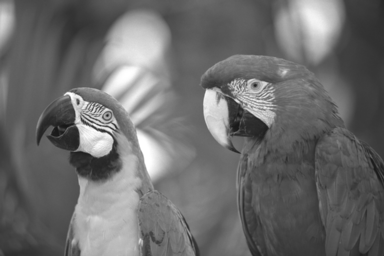
\includegraphics[width=1\textwidth]{../img22gd2.png}
    \begin{center}
    \end{center}
\end{figure}
\subsection{Print out of image showing the connected set for s = (67, 45), and T = 2}
\begin{figure}[H]
    \centering
    
\includegraphics[width=1\textwidth]{../connected-set-2t.png}
    \begin{center}
    \end{center}
\end{figure}
\subsection{Print out of image showing the connected set for s = (67, 45), and T = 1}
\begin{figure}[H]
    \centering
    
\includegraphics[width=1\textwidth]{../connected-set-1t.png}
    \begin{center}
    \end{center}
\end{figure}
\subsection{Print out of image showing the connected set for s = (67, 45), and T = 3}
\begin{figure}[H]
    \centering
    
\includegraphics[width=1\textwidth]{../connected-set-3t.png}
    \begin{center}
    \end{center}
\end{figure}
\subsection{C Code}
\lstinputlisting[language=C]{../section1.c}



\section{Image Segmentation}
\subsection{Print out of randomly colored segmentation for T = 1, T = 2, and T = 3}
\begin{figure}[H]
    \centering
    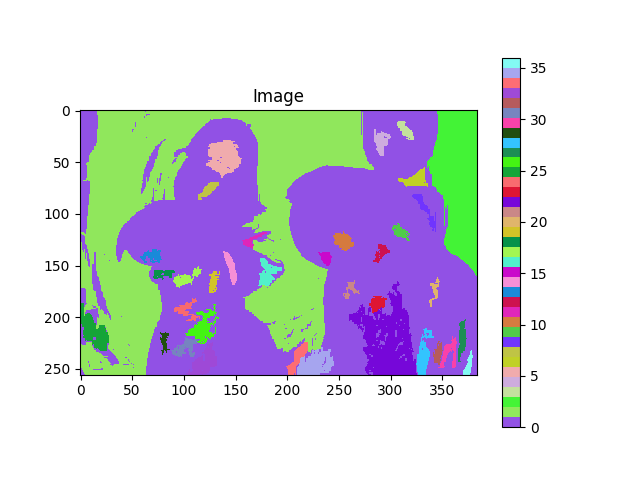
\includegraphics[width=1\textwidth]{../segmentation-1t-contrasted.png}
    \caption{T = 1}
    \begin{center}
    \end{center}
\end{figure}
\begin{figure}[H]
    \centering
    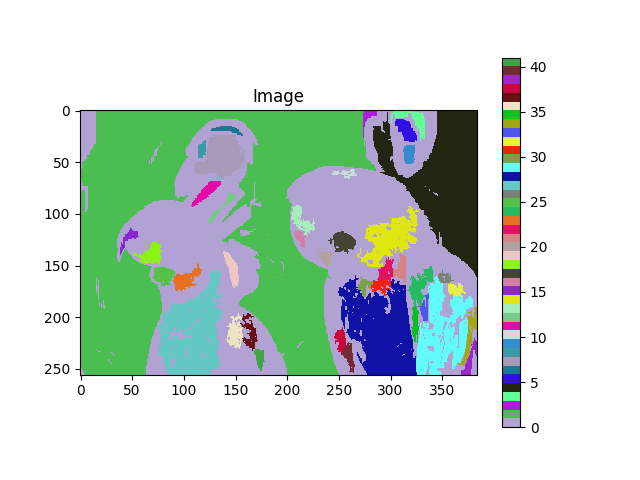
\includegraphics[width=1\textwidth]{../segmentation-2t-contrasted.png}
    \caption{T = 2}
    \begin{center}
    \end{center}
\end{figure}
\begin{figure}[H]
    \centering
    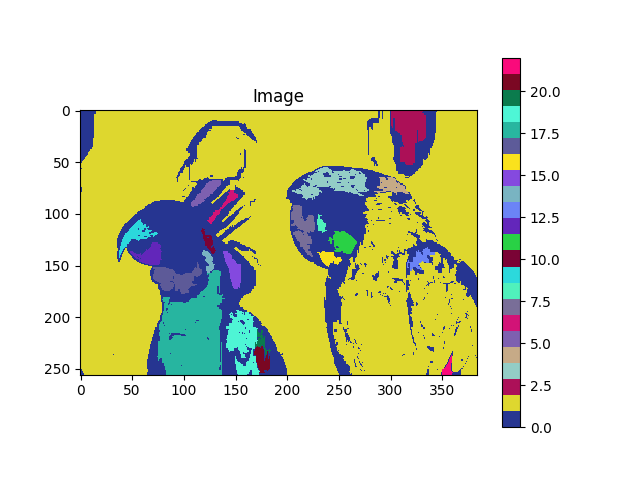
\includegraphics[width=1\textwidth]{../segmentation-3t-contrasted.png}
    \caption{T = 3}
    \begin{center}
    \end{center}
\end{figure}

\subsection{Listing of the number of regions generated for each of the values of T = 1, T = 2, and T = 3}
\begin{center}
    % T | Total segments | Large Segments
    \begin{tabular}{|c|c|c|}
        \hline
        T & Total Segments & Large Segments \\
        \hline
        1 & 27654 & 36 \\
        \hline
        2 & 16747 & 41 \\
        \hline
        3 & 11190 & 22 \\
        \hline
    \end{tabular}
\end{center}

\subsection{C Code}
\lstinputlisting[language=C]{../section2.c}



\section{Appendix - util.c Code}
Below is the code included in util.c. All other function calls not included in any of the source codes in this document are available in the starter code provided in lab 1.
\lstinputlisting[language=C]{../util.c}

\end{document}
